\documentclass{standalone}
\usepackage{tikz, fkmath}
\begin{document}
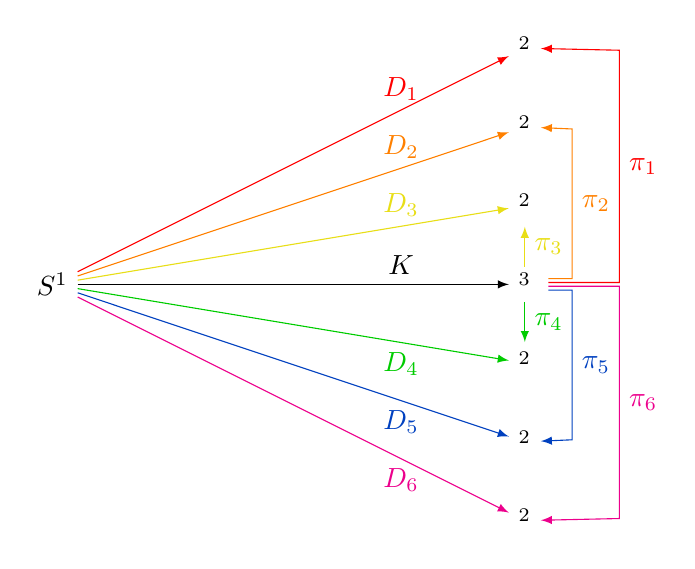
\begin{tikzpicture}

  \pgfmathsetmacro{\xgap}{3}
  \pgfmathsetmacro{\ysep}{.05}
  \pgfmathsetmacro{\xsep}{.6}

  \node (S1) at (-\xgap,0) {$S^1$};

  \node (R3) at (3,0) {$\RR^3$};

  \draw[-latex] (S1) -- (R3) node[above, near end] {$K$};
  % \draw[-latex] (R3)

  % \node (idkwhattocallthis) at (\xsep, 0) {};

  \foreach \y/\n in {3/1,2/2,1/3,-1/4,-2/5,-3/6}{
    \node (R2\n) at (\xgap,\y) {$\RR^2$};
  }


  \begin{scope}[yshift=-.75]
    % R3
    \draw[-latex, yellow!90!black] (3, 5*\ysep) -- (R23)
    node[midway, right] {$\pi_3$};
    \draw[-latex, yellow!90!black] (S1) -- (R23) node[near end, above] {$D_3$};

    % R2
    \draw[-latex, orange] (3.3, 2*\ysep) -- (3+\xsep, 2*\ysep) -- (3+\xsep, 2)
    node[midway, right] {$\pi_2$} -- (R22) ;
    \draw[-latex, orange] (S1) -- (R22) node[near end, above] {$D_2$};


    % R1
    \draw[-latex, red] (3.3, 1*\ysep) -- (3+2*\xsep, 1*\ysep) --
    (3+2*\xsep, 3) node[midway, right] {$\pi_1$} -- (R21);
    \draw[-latex, red] (S1) -- (R21) node[near end, above] {$D_1$};
  \end{scope}
  % Liftoff!

  \begin{scope}[yshift=.75]
    % R4
    \draw[-latex, green!80!black] (3, -5*\ysep) -- (R24)
    node[midway, right] {$\pi_4$};
    \draw[-latex, green!80!black] (S1) -- (R24) node[near end, below] {$D_4$};
    % R5
    \draw[-latex, blue!75!green] (3.3, -2*\ysep) -- (3+\xsep,
    -2*\ysep) -- (3+\xsep, -2) node[midway, right] {$\pi_5$} -- (R25);
    \draw[-latex, blue!75!green] (S1) -- (R25) node[near end, below] {$D_5$};
    % R6
    \draw[-latex, magenta] (3.3, -1*\ysep) -- (3+2*\xsep, -1*\ysep) --
    (3+2*\xsep, -3) node[midway, right] {$\pi_6$} -- (R26);
    \draw[-latex, magenta] (S1) -- (R26) node[near end, below] {$D_6$};
  \end{scope}


  % \draw[-latex] (S1) -- (R2) node[above, midway] {$D$};
  % \draw[-latex] (S1) -- (R3) node[below left, midway] {$K_1$};
  % \draw[-latex] (R3) -- (R2) node[below right, midway] {$\pi_1$};


  % \foreach \y/\n in {1/3, 2/2, 3/1}{
  %   \node (R32) at (0,\y) {$\RR^3$};
  %   \draw[-latex] (S1) -- (R32) node[below right, xshift=-5pt, near end] {$K_\n$};
  %   \draw[-latex] (R32) -- (R2) node[below left, xshift=5pt, near start] {$\pi_\n$};
  % }
  % \foreach \y/\n in {-3/6, -2/5, -1/4}{
  %   \node (R32) at (0,\y) {$\RR^3$};
  %   \draw[-latex] (S1) -- (R32) node[above right, xshift=-5pt, near end] {$K_\n$};
  %   \draw[-latex] (R32) -- (R2) node[above left, xshift=5pt, near start] {$\pi_\n$};
  % }

\end{tikzpicture}
\end{document}
